\documentclass[conference]{IEEEtran}
% \documentclass{sig-alternate}

\usepackage{xspace}
\usepackage{graphicx}
% \DeclareGraphicsExtensions{.pdf,.jpeg,.png}
% \usepackage{url}
%\usepackage[procnames]{listings}
\usepackage{paralist}
\usepackage{listings}
\usepackage{xcolor}
\usepackage{url}


% *** SOURCE CODE LISTINGS ***
\usepackage{paralist}
\usepackage{listings}
\usepackage{xcolor}

\lstdefinelanguage{conesc}
{
 morekeywords={components, is, case, switch, if, return, error, default, context, group, layered, command, module, interface, implementation, contexts, event, call, void, uses, transitions, triggers, iff, activate},
 morecomment=[s]{/*}{*/},
 sensitive=false,
 escapeinside={*}{*}
 \setcounter{lstNoteCounter}{0}
}

\lstset{
  basicstyle=\scriptsize\ttfamily,
  keywordstyle=\bfseries,
  showstringspaces=false,
  emphstyle=\bfseries,
}

\definecolor{Lemon}{HTML}{FFFACD}
\lstdefinestyle{conescframe}{
  language=conesc,
  frame=lines,%single,
  xleftmargin=4mm,
  framexleftmargin=4mm,
  numbers=left,
  numberstyle=\scriptsize,
  numbersep=4pt,
  backgroundcolor=\color{Lemon}
}

\usepackage{xspace}
\newcommand{\conesc}{{\textsc{ConesC}}\xspace}
\newcommand{\code}[1]{{\bfseries\texttt{#1}}}
\newcommand{\lm}[1]{\footnote{{\bf Luca: #1}}}
\newcommand{\ma}[1]{\footnote{{\bf Mike: #1}}}
\newcommand{\fakepar}[1]{\vspace{0mm}\noindent\textbf{#1.}}

% -begin- //nice in-code glyphs routine
\usepackage{tikz}
% for the pretty dark-circle-enclosed numbers
\newcommand*\circled[2]{
  \resizebox{14.5pt}{!}{
    \tikz[baseline=(char.base)]{
      \node[shape=circle,fill,inner sep=0.1pt, text=white,font=#2] (char) {#1};
    }
  }
}

\newcounter{lstNoteCounter}
\newcommand{\lstref}[1]{\hspace{-5pt}\hbox to 14.5pt{\circled{\ref{#1}}{\normalsize}}}
\newcommand{\lstnote}[1] {
  \label{#1}\hbox to -8.5pt{\llap{{\circled{\ref{#1}}{\scriptsize\rmfamily}}}}
}
% -end- //nice in-code glyphs routine

% -begin- // figures template
\usepackage{subfig}
\usepackage{xkeyval}
\usepackage{realboxes}
\makeatletter
\define@key{putfigure}{caption}{\def\pf@caption{#1}}
\define@key{putfigure}{label}{\def\pf@label{#1}}
\newcommand*\putfigure[2]{
 \setkeys{putfigure}{#1}
 \begin{figure}[!tb]
  #2
  \vspace{-4mm}
  \caption{\pf@caption}
  \label{\pf@label}
  \vspace{-5mm}
 \end{figure}
}
\define@key{putsnippet}{boxname}{\def\ps@boxname{\csname #1\endcsname}}
\define@key{putsnippet}{caption}{\def\ps@caption{#1}}
\define@key{putsnippet}{label}{\def\ps@label{#1}}
\newcommand*\putsnippet[1]{
 \setkeys{putsnippet}{#1}
 \putfigure{caption=\ps@caption,label=\ps@label}{
    \usebox{\ps@boxname}
 }
}
\makeatother
% -end- // figures template

% correct bad hyphenation here
\hyphenation{op-tical net-works semi-conduc-tor}


%No space between bibliography items:
\let\oldthebibliography=\thebibliography
  \let\endoldthebibliography=\endthebibliography
  \renewenvironment{thebibliography}[1]{%
    \begin{oldthebibliography}{#1}%
      \setlength{\parskip}{0ex}%
      \setlength{\itemsep}{0ex}%
  }%
  {%
    \end{oldthebibliography}%
  }

\begin{document}

\title{Towards Context-oriented Self-adaptation in\\Resource-constrained Cyberphysical Systems}

% Author names and affiliations
% use a multiple column layout for up to two different
% affiliations


% author names and affiliations
% use a multiple column layout for up to three different
% affiliations
\author{
\IEEEauthorblockN{Mikhail Afanasov}
\IEEEauthorblockA{Politecnico di Milano, Italy\\
afanasov@elet.polimi.it}
\and
\IEEEauthorblockN{Luca Mottola}
\IEEEauthorblockA{Politecnico di Milano, Italy and \\
SICS Swedish ICT\\
luca.mottola@polimi.it}
\and
\IEEEauthorblockN{Carlo Ghezzi}
\IEEEauthorblockA{Politecnico di Milano, Italy\\
carlo.ghezzi@polimi.it}}

% \author{ 
% \alignauthor 
% %
% M.~Afanasov$*$, L. Mottola$*\dagger$ and C.~Ghezzi$*$\\
% %
% \affaddr{$*$Politecnico di Milano (Italy), $\dagger$SICS Swedish ICT} \\
% }

% make the title area
\maketitle

\begin{abstract}
  We present a context-oriented approach to develop self-adaptive
  software for extremely resource-constrained cyber-physical systems
  (CPSs). % These are sensing and actuating systems deployed in the
  % physical world whose operation is controlled by a computing and
  % communication core.
  Because of unpredictable environment dynamics, CPS software must be
  designed and implemented to dynamically adapt to widely different
  situations. Our approach provides design concepts and language
  support to achieve this against extreme resource constraints. To
  this end, we bring a notion of context-oriented design and
  programming down to platforms with only a few KBytes of memory and
  currently leveraging rather basic programming environments. Early
  results demonstrate that our approach greatly simplifies the design
  and implementation of adaptive CPS software at the price of a modest
  system overhead. To our knowledge, we are the first to enable
  context-oriented design and programming in similarly-constrained
  platforms.
\end{abstract}


%%% Local Variables: 
%%% mode: latex
%%% TeX-master: "paper"
%%% End: 


\section{Introduction}

Cyberphysical systems (CPSs) gather data from and take actions on the real
world. The environmental dynamics determines the requirement for CPS software to
be adaptable. Moreover, adaptation should occur simultaneously along diferent
dimensions. In wildlife tracking applications~\cite{pasztor10:selective}, for
example, sensor nodes are attached to animals to study their movements, social
interactions, and health conditions. Nodes are running on batteries, which makes
the energy a precious resource. To save it, such devices as GPS and radio should
be disabled when not needed. Orthogonally, the node should send the data to the
base-station, if it is reachable, or save it locally otherwise.

In the absence of design-time support for self-adaptive software, the adaptation
described above would be achieved by ad-hoc
code~\cite{Zimmerling12,Bourdenas11}, that makes the application cumbersome to
design, and difficult to understand, debug, and maintain. A more general
approach -- context-oriented programming (COP)~\cite{Hirschfeld08} -- addresses
these issues by providing a design-time abstractions for adaptations. There are
many implementations of COP in high-level
languages~\cite{Ghezzi10,Salvaneschi12,Sehic11}, most of which are not
applicable to embedded systems, because of resource limitations.

%Many works exist in the area of self-adaptive embedded
%systems~\cite{Zimmerling12,Bourdenas11}, which illustrates a problem-specific
%approach dedicated code. A more general approach -- context-oriented
%programming (COP)~\cite{Hirschfeld08} -- is implemented in several high-level
%languages~\cite{Ghezzi10,Salvaneschi12,Sehic11}. Most of them are not
%applicable to the embedded systems, because of resource limitations.

By borrowing COP concepts and bringing them down to low-level CPS software, we
provide a design-time and programming support to enable self-adaptive behavior.
As a result, we introduce \conesc -- a context-oriented extension of nesC
language -- in Sec.~\ref{sec:concepts}, where we also describe the concepts the
language was build upon. We discuss our preliminary evaluations in
Sec.~\ref{sec:eval}, and open problems in Sec.~\ref{sec:future}.

\section{Design Concepts}
\label{sec:design}

Our approach to support the design of self-adaptive CPS software is
intentionally fundamental and conceptually simple. However,, the lack
of a principled approach for its design is currently hampering the
field at large~\cite{Picco:2010:SEW:1882362.1882421}. Key in our
approach is the combination of design-time support and programming
model. We illustrate the latter in Section~\ref{sec:conesc}.

We define two key design concepts: \emph{i)} individual
\emph{contexts}; and \emph{ii)} \emph{context groups}, along with the
notions necessary to weave these concepts into a complete design.
Contexts represent the different environmental situations the system
may encounter, and correspond to behavioral variations associated to a
given situation. As the environment surrounding the system mutates,
the software adapts accordingly by \emph{activating} a suitable
context. Context groups represent collections of individual contexts
sharing common characteristics; e.g., whenever the \emph{same}
functionality must adapt to changes in the surrounding environment.

\begin{figure}
\begin{center}
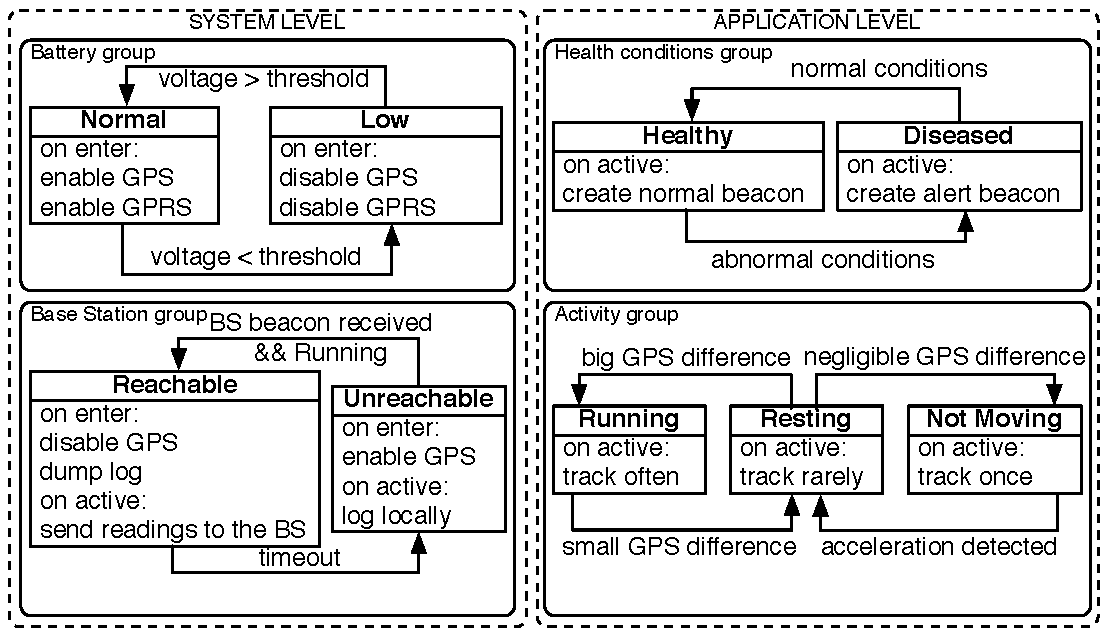
\includegraphics[scale=.45]{imgs/wildlifetracking}
\vspace{-4mm}
\caption{Wildlife monitoring application design.}
  \label{fig:design}
\vspace{-6mm}
\end{center}
\end{figure}

Figure~\ref{fig:design} graphically depicts the context-oriented
design of the example wildlife monitoring applications described
earlier. Context groups are defined to describe behavioral variations
corresponding to battery levels, base-station reachability, as well as
an animal's health conditions and activity. Context groups are tagged
as system-level or application-level to discern application-specific
functionality from likely re-usable system services.

The contexts within a group define the behavioral variations at
hand. For example, the software must behave differently depending on
whether the base-station is reachable.  The contexts in a group are
tied with explicit \emph{transitions}, labeled with the conditions
triggering the context change. For example, within the
``Base-station'' group, the system transitions from context
``Reachable'' to ``Unreachable'' whenever no beacons are received from
the base-station within a specific timeout. This entails a node is out
of the base-station communication range and the software must adapt
accordingly; for example, by locally storing the contact logs instead
of sending them over the radio.

The specific software adaptation is encapsulated in the individual
contexts. In the latter, it is useful to distinguish \emph{one-time
operations} executed at the time of entering or existing a context,
from \emph{continuous activities} that occur as long as a context is
active. For example, whenever entering ``Reachable'', the software
dumps on the base-station the contact logs locally accumulated while
the latter was unreachable. Similarly, when in the latter situation, the
software must log the contacts locally as long as ``Base-station
unreachable'' persists, as shown in Figure~\ref{fig:design}.

The required adaptation functionality may span multiple context
groups. To this end, developers can bind context activations across
groups. An example is in the ``Reachable'' context within the
``Base-station'' group: when entering, ``Not Moving'' must also
consequently activate. As base-stations are typically deployed at
known locations, and yet their radio range is very limited,
continuously sampling the GPS is likely a waste of energy, and we can
avoid waiting for the next sample before deciding that we can stop
sampling until an acceleration is detected.

Developers may also make context transitions subject to the activation
of other contexts, which is useful to check for design errors at
run-time. An example is when activating ``Diseased'' in the ``Health
conditions'' group. Besides an abnormal body temperature that may
reveal a disease, the adaptation process must check that either
``Resting'' or ``Not Moving'' in the ``Animal activity'' group is
currently active. Indeed, if an animal is diseased, it is probably not
very active. Should that not be the case, developers might have not
correctly captured how contexts evolve, potentially indicating a
design error.

The concepts we define provide design-time support to reason on the
different situations the software must adapt to, and to identify common
functionality, orthogonal aspects, and mutual constraints. This
ultimately helps separate concerns during the implementation phase, as
we illustrate next.



%%% Local Variables: 
%%% mode: latex
%%% TeX-master: "paper"
%%% End: 

\section{Programming Support}
\label{sec:conesc}

We directly render the design concepts above in a set of programming
constructs feasible within existing programming environments for
resource-constrained CPS platforms. In doing so, we borrow from
context-oriented programming (COP)~\cite{}. We exemplify our approach
based on nesC~\cite{}, a mainstream sensor network programming
language. However, our approach is not tied to it, and may be readily
translated to other programming systems~\cite{programmingsurvey}.

\fakepar{Target language} nesC is an event-driven programming language
for sensor networks, derived from C. Applications are built by
interconnecting \emph{components} that interact by providing or using
\emph{interfaces}. An interface lists one or more functions, tagged as
\emph{commands} or \emph{events}. Commands are used to execute
actions, while events are used to collect the results
asynchronously. % Interfaces in nesC are bidirectional: data flows both
% ways between components connected through the same
% interface.
Component \emph{configurations} specify the wirings among
components. % Configurations are component themselves, so they can offer
% interfaces and be wired to other components.

nesC exemplifies the limitations dictated by the extreme resource
constraints of the target platforms, and hence the reasons why
existing COP approaches cannot be directly ported. Because of the few
KBytes of memory typically available, for example, components cannot
be instantiated at run-time. They are rather in-lined at compile time
so the compiler can reduce the size of the executable
binary~\cite{nesc}, which would hardly fit in the available program
memory otherwise. The use of dynamically-allocated memory is extremely
discouraged: the MCUs provide no memory protection while the systems
are meant to be long-running, so bugs in memory handling may have
disastrous effects and yet be very difficult to nail down.


\begin{figure}[!tb]
\begin{lstlisting}[style=conescframe]
context group BaseStationG {
 layered command void report(contact_t contact); *\label{cg:layered}*
}implementation {
 contexts Reachable, Unreachable is default, *\label{cg:ctx}* 
          ErrorC is error; *\label{cg:error}*
 // Standard nesC component wirings...
}
\end{lstlisting}
\vspace{-4mm}
\caption{Context group in \conesc.}
  \label{fig:configuration}
\vspace{-2mm}
\end{figure}

\fakepar{\conesc} Notwithstanding the above constraints, we design a
context-oriented extension to nesC, called \conesc, that incorporates
the design concepts described in Section~\ref{sec:design}.

A \code{context group} in \conesc extends the standard nesC
configurations by specifying, in addition to component wirings, the
contexts included in the group and the \emph{layered
  functions}~\cite{cop} that such contexts provide. The latter are
functions whose behavior depends on the currently active context, and
are hence the primary means to implement the behavioral variations
necessary for self-adaptation. The individual contexts, which extend
the standard notion of nesC component, provide the individual
environment-dependent implementations of layered functions.

Figure~\ref{fig:configuration} depicts a snippet of \conesc code to
implement the ``Base Station'' group in Figure~\ref{fig:design}. In
this example, the \code{report()} function (line~\lstref{cg:layered})
changes behavior depending on whether the base-station is
\code{Reachable} or \code{Unreachable}. The latter are the contexts
included in this group, specified after the keyword \code{contexts}
(line~\ref{cg:ctx}) with optional modifiers to specify the active
context at start-up (\code{is default} in line~\ref{cg:ctx}) and an
error context (\code{is error} in line~\ref{cg:error}). The error
context is automatically activated should there be violations to
constraints defined over context transitions, e.g., the fact that
``Running'' must be active when transitioning from
``Unreachable'' to ``Reachable'', as shown in Figure~\ref{fig:design}.

\begin{figure}[!tb]
\begin{lstlisting}[style=conescframe]
context Unreachable {
 transitions Reachable iff ActivityG.Running; *\label{ct:tr}*
 uses interface DataStore;
} implementation {
 event void activate(){ //...} *\label{ct:activate}*
 event void deactivate(){ //...} *\label{ct:deactivate}*
 layered command void report(contact_t contact){ *\label{ct:layer}*
  call DataStore.deposit(contact);
 }
}
\end{lstlisting}
\vspace{-4mm}
\caption{Individual context in \conesc.}
  \label{fig:context}
\vspace{-2mm}
\end{figure}

Figure~\ref{fig:context} shows the \conesc specification of the
``Unreachable'' context. The keyword \code{transitions}
(line~\ref{ct:tr}) specifies the allowed outgoing transitions,
possibly with associated constraints expressed with the \code{iff}
keyword. The specific implementation of the layered function is
indicated with the \code{layered} keyword
(line~\ref{ct:layer}). Command and event implementations are as in
standard nesC. Particularly, the predefined events \code{activate()}
(line~\ref{ct:activate}) and \code{deactivate()}
(line~\ref{ct:deactivate}) are automatically signalled when entering
and existing the context, allowing the implementation of one-time
operations and the start/stop of continuous activities in a context.

Explicit context activation may happen anywhere in the code, using the
\code{activate} keyword, as in
\begin{lstlisting}[language=conesc]
activate BaseStationG.Unreachable;
\end{lstlisting}
Notably, this allows to completely decouple the context-dependent
application logic---confined within the layered functions inside the
individual contexts---from the adaptation logic itself, which may be
specified in a separate component. 

Additionally, a keyword \code{triggers} to be used close to
\code{transitions} in an individual context is available to bind
context activations across groups, as in the case of ``Low'' in
Figure~\ref{fig:design}, which is required to consequently activate
``Unreachable''.\lm{CHECK!}

%%% Local Variables: 
%%% mode: latex
%%% TeX-master: "paper"
%%% End: 

\section{Evaluation}\label{sec:eval}

For evaluation purposes, we implemented three applications. For each we compare
nesC implementation against its \conesc counterpart.

{\bf Complexity} is estimated by using such metrics as the number of lines of
code (LOC), the number of variables declared and functions
defined~\cite{Pressman01}. Despite our results show 30\% increase of average
complexity, there is significant reduction in average per-module complexity --
-54\%. We believe that in larger applications the number of the similar lines of
code will be bigger. Nevertheless, \conesc-written applicaton is more than 3
times smaller than generated code, what makes \conesc an effective tool for
context-oriented programming.

{\bf Overhead} in terms of memory is lesser than
2,5\% for binary size and less than 4,5\% for RAM overhead. The average CPU
overhead for layered function calls oscillates from 2 to 5 CPU cycles depending
on application, which is negligible in terms of energy consumption, since the
simplest operation in TinyOS -- turn on/off LEDs -- consumes 8 CPU cycles. The
context transitions overhead is bigger -- from 10 to 25 CPU cycles -- but
remains in the same order of magnitude.

\section{Emerging Patterns}
\label{sec:patterns}

Despite the limited experience we hitherto gathered using \conesc, we
already observe quite distinctive design and programming patterns,
representing solutions to commonly occurring problems. In general,
however, they cannot be directly transformed into executable code
without proper application-specific implementations.

% \conesc, as we mentioned before, makes the components of application more
% decoupled and reusable. To show that, we provide three possible patters --
% general solutions to a commonly occurring problems. 

\fakepar{Behavior control} Programmers often employ a single context
group to specify different behaviors for the same high-level
functionality. One such example is the ``Base-station'' group in
Figure~\ref{fig:design}, which includes two different behaviors for
the functionality to report contact logs to the users. The
functionality itself is exported by one or more layered functions
defined in the group. The chosen behavior is then determined by
activating a single context within the group.

We found similar designs in other applications as well. In the
adaptive protocol stack, for example, the packet relay functionality
also matches a similar design. Depending on a node's mobility, the
chosen behavior is picked out of a pool of available protocols, whose
functionality are encapsulated in single contexts. These are in turn
included in a single context group, which exports a layered function
where the application layers transparently accesses whatever protocol
is in operation at a given time.

% Whenever the application should perform some specific
% actions repeatedly, according to the environmental conditions, the developer
% should use \emph{Behavior Control Pattern}. The example is in our scenario, when
% the application adapts to the reach-ability of the base-station.

Figure~\ref{fig:control} shows an abstract view of such commonly
recurring pattern. In addition to the context group exporting the
adaptive functionality and the single contexts therein, programmers
also define an additional ``controller'' component, which activates
the single contexts within the group depending on the
situation. Figure~\ref{fig:bscm} shows one such example for the
wildlife monitoring application. Similar designs apply to the
smart-home controller and the adaptive protocol stack as well.

\begin{figure}
\begin{center}
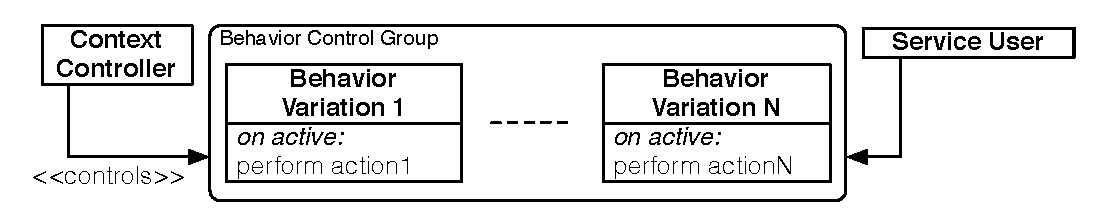
\includegraphics[scale=.43]{imgs/beh_var}
\vspace{-1mm}
\caption{Behavioral control pattern.}
  \label{fig:control}
\vspace{-8mm}
\end{center}
\end{figure}

% Context group in that case includes the functionality, which needs to adapt.
% Each context implies an implementation of a corresponding functionality. 

% To make the pattern complete, we also use a separate control module,
% which is responsible only for the activating suitable context in the
% given context group. Since this pattern controls the behavior of the
% device, it is mostly applicable in the system level.

% Behavior Control Pattern can also be applied on Smart-home system, when system
% needs to send data to the Fire, or Police, or both, depending on the type of
% emergency. The Adaptive protocol can also use this pattern to switch between
% CTP- or Gossip-based protocols depending on the network topology.

\fakepar{Content provider} Different from the behavior control
pattern, which provides non-trivial context-dependent processing, we
observe cases where context-dependent \emph{data} is offered to other
functionality with little to no processing involved. In the wildlife
monitoring application, for example, the ``Health conditions'' group
in Figure~\ref{fig:design} provides differently formatted beacons to
the radio driver for broadcast transmissions. Layered functions are,
in this case, defined for the group merely to retrieve the
context-dependent data.

In this case as well, we notice the same pattern in other
applications. In the smart-home controller, for example, a context
group is defined to manage the user preferences depending on day vs.\
night. These data are simply retrieved differently from a common data
storage by two different contexts modeling day or night
situations. Whatever user preference is to be considered at a given
point is then handed over to the control loop in charge of setting the
functioning of the climate systems.

\begin{figure}
\begin{center}
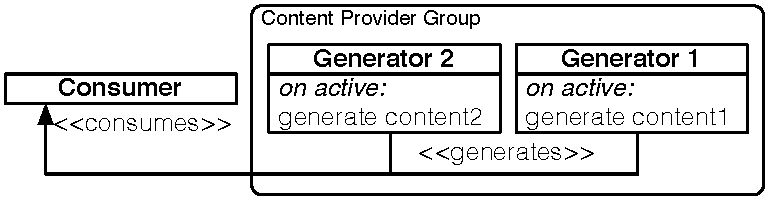
\includegraphics[scale=.43]{imgs/content_provider}
\vspace{-1mm}
\caption{Content provider pattern.}
  \label{fig:provider}
\vspace{-8mm}
\end{center}
\end{figure}

In abstract terms, this pattern's structure differs from that of
behavior control in that the role of the ``controller'' component is
often fairly trivial. In the smart-home controller, for example, the
controller component is simply based on the time of the day. On the
other hand, the component consuming the context-dependent data plays a
key role. Indeed, while functionality structured according to behavior
control can be considered stand-alone, the context provider needs to
be tailored to the data consumer component.

\fakepar{Trigger} We also recognize designs where single contexts are
used only to trigger specific operations when entering/exiting a
context, but no significant context-dependent functionality or data is
offered as the same context remains active. One example in the wildlife
monitoring application is the ``Battery'' group in
Figure~\ref{fig:design}. The included contexts are used to
enable/disable the GPS sensor depending on battery levels, but no
other functionality is provided to other components. In this
case, layered functions are often not defined, in
that the predefined \code{activated} and \code{deactivated} events
within the single contexts suffice.

In the smart-home controller, for example, we notice a similar pattern
in the context group regulating light dimming. Depending on
perceived light levels in a room, either context ``Too bright'' or
``Too dark'' is activated, and lights are tuned accordingly when
entering either context. This processing is entirely implemented
within the corresponding \code{activated} event handlers. 

In more general terms, a ``controller'' component is present in this
case as well to drive the context transitions in the group. However,
unlike the other patterns, there is no other component that either
uses context-dependent functionality or consumes context-dependent
data.

\begin{figure}
\begin{center}
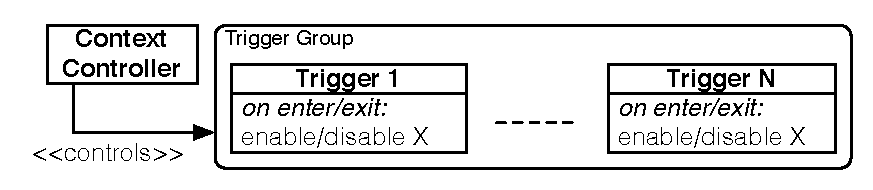
\includegraphics[scale=.43]{imgs/con_act}
\vspace{-1mm}
\caption{Trigger pattern.}
  \label{fig:trigger}
\vspace{-8mm}
\end{center}
\end{figure}

%%% Local Variables: 
%%% mode: latex
%%% TeX-master: "paper"
%%% End: 

\section{Related Work}
\label{sec:related}

Efforts close to ours particularly address the design and
implementation of self-adaptive embedded system software,
context-oriented programming, and system-level adaptiveness in
CPSs. We briefly survey paradigmatic examples.

Works in self-adaptive embedded system software
cover contributions from requirement engineering to
verification~\cite{cheng:adaptive}. Co-design approaches also exist
where the hardware/software boundaries blur for greater
flexibility~\cite{diguet11:closed}. Unlike in our work, several of
these solutions focus on a few environmental dimensions, each
requiring ad-hoc self-adaptive functionality. In our target
applications, complexity arises especially from the several
combinations that multiple environmental dimensions concurrently
generate. Nevertheless, most of these solutions would be hardly
applicable in resource-constrained CPSs, due to
run-time overhead.

Villegas~\cite{VilegasPhD11} designed dedicated software support for
situation-aware software systems. Despite sharing some high-level
challenges with our work, Villegas relies on the end-user as a
controller of context management, whereas we focus on autonomous
systems. Moreover, we directly deal with physical sensors to acquire
context information, whereas these are abstracted in software-based
sensor devices in Villega's work.

% e.g. adaptivity and context representation and management -- are
% addressed in the work, the motivating example and consequent reasoning
% are base on user-centric self-adaptive software systems. The latter
% implies the end-user as a controller of the context management, while
% we are focused on the systems which are governed by themselves, or by
% the programmer, at least. The proposed in~\cite{VilegasPhD11} context
% ontology, context control model and reference model are not
% considering application scenarios of CPSs, and, thus, are not
% applicable. Differently, our research is based on particular
% challenges arose when creating adaptive software for CPSs. Besides, we
% are using physical sensor devices and considering all the consequent
% challenges to derive the context, while Villegas
% N.~\cite{VilegasPhD11} is considering software-based \emph{sensor} to
% monitor software service interface.

Fleurey et al.~\cite{Fleureya-adaptive-firmwares11} present a
model-driven approach for creating adaptive firmwares. They model the
application as a single state machine and define behavioral variations
based on predicates defined over the application state. When such
predicates are found true, the system accordingly adapt the state
machine transitions. Code is automatically generated from these
specifications. Compared to this effort, we do not target completely
automatic code generation, but provide dedicated programming
constructs. This offers greater freedom in encoding the conditions to
trigger context changes and enables finer-grained optimizations, which
may be mandatory given the resource limitations. Moreover, we seek to
integrate our approach in existing component-based CPS frameworks,
leveraging the existing code base.

The COP model~\cite{Hirschfeld08} is implemented in several high-level
languages~\cite{Bardram05,Ghezzi10,Kamina11,Salvaneschi12,Sehic11}. These
are, however, generally unfeasible on the platforms we target. We
borrow a few of these concepts---for example, our layered functions in
context groups are akin to the concept of
layer-in-class~\cite{Salvaneschi12}---and adapt them to the
limitations of component-based frameworks for resource-constrained
CPSs. In this area, the embedded devices are rather seen as
application-agnostic providers of raw sensor
data~\cite{Sehic11}. Differently, we bring COP down to the
component-based CPS software, enabling self-adaptive functionality
right on the devices that directly interact with the environment.

Aside from COP, Meta- and Aspect-oriented Programming (AOP) offer
programming support to implement adaptive
functionality~\cite{SalvaneschiTBP}. The former requires
self-modification of the binary, which is often unfeasible in
resource-constrained CPSs. Similar requirements hold for
AOP~\cite{Kiczales:AOP:97}, which is often applied to large complex
software projects. Arguably, applying AOP to the relative simple
processing running aboard the CPS devices, even if possible, would be
quite overkill.

% was introduced to handle the
% crosscutting in concerns of software. Each software has a number of
% orthogonal functionality -- e.g. concerns -- which might intersect
% each other in some parts of the
% source-code~\cite{Tarr:concerns:99}. To keep modularization and
% maintainability, AOP allows to separate these parts into the
% \emph{aspects}, and, thus, to save the separation between
% concerns. COP, however, focuses on the representation of alternative
% behavior, by using notion of \emph{layers} and separating the
% implementations of behavioral variations.  Thus, the separation into
% aspects is no more needed. Moreover, among the other mentioned
% techniques, COP yields programs with the lowest
% complexity~\cite{SalvaneschiTBP}.

Specific cases of run-time adaptation are seen at system level in the
CPS literature. For example, Zimmerling et al.~\cite{zimmerling12}
focus on run-time reconfiguration of MAC protocol parameters depending
on environmental conditions. Routing protocols expressly designed with
self-adaptive functionality also exist~\cite{Bourdenas11}. Such
efforts essentially address a complementary problem. While we aim to
provide design-time and programming support to implement self-adaptive
software in this domain, these works focus on the actual
problem-specific adaptation logic.

% There are some attempts to apply context-oriented programming for the software
% for CPSs. Sehic et al.~\cite{Sehic11}, for example, proposed a macro-language
% for rapid development of context-aware applications for CPSs. Wood et
% al.~\cite{Wood08} developed a CPS for Assisted-Living and Residential
% Monitoring, which utilizes a technique of a context-depended behavior. Another
% work, provided by Ghezzi et al.~\cite{}, is devoted to the language
% support for bringing a context-awareness for CPSs.

% Several attempts were also performed towards self-adaptive software for CPSs. In
% the work of Steine et al.~\cite{Steine11} authors were focused on run-time
% reconfiguration of WSNs by adjusting protocol values dynamically depending on
% the conditions the system operates in. Marques et al.~\cite{Marques11} propose a
% run-time evaluation of QoS characteristics for better adaptation. Another
% research was provided towards self-adaptive protocols: MAC-protocol by Park et
% al.~\cite{Park08} and routing protocol by Bourdenas et al.~\cite{Bourdenas11}.
% Self-adaptivity is also considered as a main ingredient of run-time error
% handling~\cite{Bourdenas10} and energy management~\cite{Jiang07}.

% Despite the research activity in the area of self-adaptive software for CPSs is
% quite intensive, it remains fragmented, and no holistic approach yet developed.
% Current research has two extreme directions:~\emph{i)} high-level software,
% which brings adaptivity only in application level using CPSs as raw-data
% providers~\cite{Wood08,Sehic11,Ghezzi10}, and~\emph{ii)} low-level software,
% which is focused on a system level ignoring an application
% level~\cite{Steine11,Marques11,Park08,Bourdenas11,Bourdenas10,Jiang07}.
% We combine different aspects of self-adaptivity for CPSs and provide robust
% approach for self-adaptivity on both system and application levels, which makes
% our work novel in this field.

% Salvaneschi et al.~\cite{SalvaneschiTBP}\footnote{to be published}\cite{Salvaneschi12} 
% outlined possible techniques for language adaptation for context-oriented
% programming. We not only utilize concepts of COP, but also provide a novel approach for
% bringing context-oriented programming to CPSs. To this end, we modified and
% applied such techniques as: \emph{Per-Object activation} and
% \emph{Layer-in-Class} \cite{Salvaneschi12}. The latter implies the
% implementations of layers~\cite{Costanza05} -- i.e. behavioral variations -- in
% one class. In our approach we used \emph{context groups} to aggregate behavioral
% variations, which are invoked by explicit activation of corresponding
% \emph{context}, i.e. we adopted \emph{Per-Object activation}, where an
% \emph{object} is a~\emph{context}.


%%% Local Variables: 
%%% mode: latex
%%% TeX-master: "paper"
%%% End: 

\section{Conclusion}
\label{sec:ending}

We presented a solution to provide design-time and programming support
for self-adaptive software in re\-sour\-ce-constrained component-based
CPS software. In this domain, the lack of a principled design approach
and the rudimentary programming environments result in entangled
implementations. To remedy this, we conceived dedicated design
concepts and COP extensions to low-level component-based CPS
frameworks. Preliminary results indicate that our approach yields
implementations that are easier to test, maintain, and evolve. The
run-time overhead to pay is, nonetheless, negligible.

% Our immediate research agenda includes automatic generation of \conesc
% code templates from graphical notations akin to
% Figure~\ref{fig:design}, and domain-specific model checking of
% context-oriented CPS applications built based on our approach.

% \hrule

As part of our research agenda, we are investigating ways to
automatically generate \conesc skeletons based on graphical
representations of contexts and context groups similar to
Figure~\ref{fig:design}. Further, we plan to use the same notation as
input to perform static verification, e.g., using domain-specific
model-checking techniques.

%%% Local Variables: 
%%% mode: latex
%%% TeX-master: "paper"
%%% End: 

% acknowledgements

% {\small
\bibliographystyle{plain}      % 
\bibliography{bibl}   % name your BibTeX data base
% }

\end{document}


